\documentclass[UTF8,a4paper,11pt,fontset=fandol]{ctexart}
\usepackage{geometry}
\geometry{margin=2.2cm}
\usepackage{amsmath,amssymb,longtable,booktabs,array,hyperref,xcolor,enumitem,graphicx,float}
\hypersetup{colorlinks=true,linkcolor=blue,urlcolor=blue}
\setlist[itemize]{leftmargin=1.3em,itemsep=0.2em}
\definecolor{notegray}{RGB}{246,248,251}
\title{P05. Hybrid Reinforcement Learning-Based Eco-Driving Strategy for Connected and Automated Vehicles at Signalized Intersections\\中英双语博士精读笔记}
\author{Zhengwei Bai; Peng Hao; Wei Shangguan; Baigen Cai; Matthew J. Barth}
\date{2022 · IEEE Transactions on Intelligent Transportation Systems}
\begin{document}
\maketitle

\noindent\textbf{Theme / 主题：} Eco-driving + hybrid RL\\
\textbf{Method family / 方法族：} Hybrid RL eco-driving at signalized intersections / 信号交叉口混合强化学习生态驾驶\\
\textbf{PDF pages / 页数：} 15 \quad
\textbf{Relevance / 相关度：} 86/100\\
\textbf{Source / 来源：} \url{https://arxiv.org/abs/2201.07833}

\section{论文全景速览与核心贡献 / High-Level Overview \& Core Contributions}
\subsection{研究背景与痛点 / Background \& Pain Points}
这篇论文位于“Eco-driving + hybrid RL”方向。对你的 JSSP-based Intersection Management 课题，它回答的是高层调度、低层轨迹平滑、安全过滤或真实验证中的一个关键子问题：如何让车辆在路口少停、少冲突、少能耗，同时保持在线可执行。

The paper belongs to the theme of Eco-driving + hybrid RL. For a JSSP-based intersection-management thesis, it illuminates one of the key layers: scheduling, smoothing, safety filtering, or real-world validation.

\textbf{Pain point / 痛点：} Signalized setting and policy-level action output differ from a scheduler-to-smoother architecture.

\subsection{核心科学问题 / Core Scientific Question}
在信号灯、V2I 信息和混合交通干扰下，如何通过混合规则-学习策略降低能耗和时间损失？

How can a hybrid rule-learning eco-driving policy reduce energy and travel time under SPaT and mixed-traffic constraints?

\subsection{科学贡献 / Scientific Contributions}
\begin{itemize}
\item 方法贡献 (method contribution)：Combines a rule-based driving manager, V2I/vision features, and RL to generate longitudinal and lateral eco-driving actions.
\item 安全/避碰贡献 (safety contribution)：Mixed-traffic policy includes rule-based safety management around surrounding vehicles.
\item 平滑/停止避免贡献 (smoothing contribution)：Targets energy and travel-time reduction by smoothing approach behavior at signalized intersections.
\item 创新力度评判 (reviewer judgement)：强应用价值：规则管理器增强 RL 安全性，适合作为轨迹平滑器能耗目标的参考。
\end{itemize}


\subsection{核心概念对照 / Core Concepts}
\begin{longtable}{p{0.24\linewidth}p{0.28\linewidth}p{0.40\linewidth}}
\toprule
中文概念 & English Concept & Role / 学术作用\\
\midrule
自动交叉口管理 & Autonomous Intersection Management & 把信号控制替换为车辆级调度与控制。 \\
轨迹平滑 & Trajectory Smoothing & 减少急加减速、停车和能耗峰值。 \\
安全约束 & Safety Constraints & 把碰撞风险写成距离、时间间隔或屏障函数。 \\
Hybrid RL eco-driving at signalized intersections & 信号交叉口混合强化学习生态驾驶 & 该论文的核心方法族。 \\
\bottomrule
\end{longtable}

\section{教材式学习路径与关键截图 / Textbook-Style Study Path \& PDF Snapshots}
\subsection{学习路径 / Study Path}
\begin{itemize}
\item 第一遍先读首页截图、摘要与引言，确认研究问题和场景假设。
\item 第二遍沿着技术路线图复现模型变量、约束和求解器输入输出。
\item 第三遍逐节阅读 section deep reading，对照 PDF 截图检查公式、图表和实验。
\item 第四遍只站在审稿人视角重读实验，判断 baseline、公平性、消融和鲁棒性。
\item 最后把博士 checklist 写成自己的复现实验或论文拓展计划。
\end{itemize}


\subsection{博士阅读 Checklist / Doctoral Reading Checklist}
\begin{itemize}
\item 能否独立重写核心公式：能耗-效率-安全复合奖励 / Energy-efficiency-safety reward，并解释每个符号的物理意义？
\item 能否画出输入-模型-算法-控制-验证的数据流图？
\item 能否指出至少两个强假设，并说明它们在真实交通中何时失效？
\item 能否复述实验基准是否公平，指标是否覆盖效率、安全、能耗和计算时间？
\item 能否提出一个与自己 JSSP/RL/smoother 课题直接相连的拓展实验？
\end{itemize}


\subsection{关键截图讲解 / PDF Snapshot Explanation}
Screenshots are selected anchors from the local PDFs for study and parallel reading. They do not replace the original paper.

\begin{figure}[H]
\centering

\includegraphics[width=0.92\linewidth]{../../assets/P05_bai2022hybrid/01_title_and_abstract_p1.jpg}
\caption{首页与摘要 / Title and abstract page (p.1, full\_page). 这张截图用于把笔记中的抽象概念拉回原论文页面，便于你平行阅读原文、公式、图表和实验设置。 与当前课题的连接：Supports the argument that stop-and-go reduction and energy-aware smoothing are important low-level objectives.}
\end{figure}

\begin{figure}[H]
\centering

\includegraphics[width=0.92\linewidth]{../../assets/P05_bai2022hybrid/02_modeling_or_problem_setup_p2.jpg}
\caption{建模或问题设定页 / Modeling or problem-setup page (p.2, full\_page). 这张截图用于把笔记中的抽象概念拉回原论文页面，便于你平行阅读原文、公式、图表和实验设置。 与当前课题的连接：Supports the argument that stop-and-go reduction and energy-aware smoothing are important low-level objectives.}
\end{figure}

\begin{figure}[H]
\centering

\includegraphics[width=0.92\linewidth]{../../assets/P05_bai2022hybrid/03_core_method_or_algorithm_p4.jpg}
\caption{核心方法或算法页 / Core method or algorithm page (p.4, full\_page). 这张截图用于把笔记中的抽象概念拉回原论文页面，便于你平行阅读原文、公式、图表和实验设置。 与当前课题的连接：Supports the argument that stop-and-go reduction and energy-aware smoothing are important low-level objectives.}
\end{figure}

\begin{figure}[H]
\centering
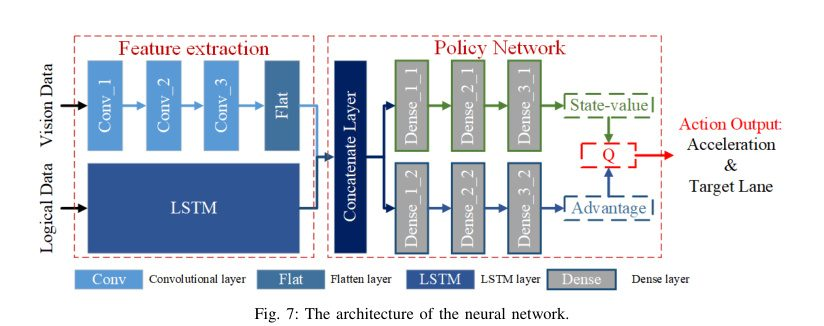
\includegraphics[width=0.92\linewidth]{../../assets/P05_bai2022hybrid/04_experiments_or_results_p9.jpg}
\caption{实验或结果页 / Experiments or results page (p.9, figure\_crop). 这张截图用于把笔记中的抽象概念拉回原论文页面，便于你平行阅读原文、公式、图表和实验设置。 与当前课题的连接：Supports the argument that stop-and-go reduction and energy-aware smoothing are important low-level objectives.}
\end{figure}

\begin{figure}[H]
\centering

\includegraphics[width=0.92\linewidth]{../../assets/P05_bai2022hybrid/05_conclusion_or_limitations_p13.jpg}
\caption{结论或局限页 / Conclusion or limitations page (p.13, full\_page). 这张截图用于把笔记中的抽象概念拉回原论文页面，便于你平行阅读原文、公式、图表和实验设置。 与当前课题的连接：Supports the argument that stop-and-go reduction and energy-aware smoothing are important low-level objectives.}
\end{figure}


\section{章节精读与逐段导读 / Section-by-Section Deep Reading \& Walkthrough}
\subsection*{p.1 I. INTRODUCTION}
\textbf{章节目标 / Learning goal：} 建立研究动机：为什么传统信号控制、FCFS 或单车控制不足以处理该论文关注的交叉口协同问题。

Understand why the paper needs a new coordination method rather than a standard signal, FCFS, or single-vehicle controller.

\textbf{关键论点 / Key argument：} 这一部分通常把痛点落到 Eco-driving + hybrid RL：既要提高效率，又要保持安全与在线可执行。

\textbf{技术焦点 / Technical focus：} 精读时标出作者批判的 baseline、场景假设、交通参与者类型和隐含优化目标。

\textbf{审稿追问 / Reviewer question：} 作者指出的痛点是否真的需要新方法，还是可以由更强的优化器/更保守规则解决？

\subsection*{p.2 II. PROBLEM FORMULATION}
\textbf{章节目标 / Learning goal：} 把自然语言交通问题压缩为变量、状态、约束、目标函数或图结构。

Translate the traffic problem into variables, states, constraints, objectives, or graph relations.

\textbf{关键论点 / Key argument：} 本节是复现论文的核心入口，应与公式“能耗-效率-安全复合奖励 / Energy-efficiency-safety reward”一起读。

\textbf{技术焦点 / Technical focus：} 逐项检查车辆状态、冲突关系、控制输入、时间/空间索引和安全阈值是否定义完整。

\textbf{审稿追问 / Reviewer question：} 这些建模假设在混合交通、通信延迟、感知误差和高密度车流下是否仍成立？

\subsection*{p.4 III. HRL- BASED ECO-D RIVING FRAMEWORK}
\textbf{章节目标 / Learning goal：} 解释算法如何把模型转化为可执行决策，并说明在线运行机制。

Trace how the paper turns the model into executable online decisions.

\textbf{关键论点 / Key argument：} 系统用规则型驾驶管理器处理安全和交通规则，用强化学习在允许动作空间中选择纵向/横向生态驾驶动作；V2I 和视觉特征帮助策略预见信号相位与周围车辆。

\textbf{技术焦点 / Technical focus：} 画出输入、核心求解器、输出和安全检查接口，明确哪些步骤是优化、哪些是规则、哪些是学习。

\textbf{审稿追问 / Reviewer question：} 若算法某一步失败，论文有没有 fallback、重规划或安全过滤机制？

\subsection*{p.4 1. On-board computer: it houses the hierarchical-RL brain}
\textbf{章节目标 / Learning goal：} 承接前后章节，补充局部定义、案例或实现细节。

Recover implementation details needed for reproduction.

\textbf{关键论点 / Key argument：} 这类章节常常不是主贡献，但决定你能否真正复现方法。

\textbf{技术焦点 / Technical focus：} 检查它是否给出了参数、伪代码、场景划分或实现细节。

\textbf{审稿追问 / Reviewer question：} 跳过该节会不会导致公式或实验无法复现？

\subsection*{p.5 2. On-board radar : As defined in previous section, three}
\textbf{章节目标 / Learning goal：} 承接前后章节，补充局部定义、案例或实现细节。

Recover implementation details needed for reproduction.

\textbf{关键论点 / Key argument：} 这类章节常常不是主贡献，但决定你能否真正复现方法。

\textbf{技术焦点 / Technical focus：} 检查它是否给出了参数、伪代码、场景划分或实现细节。

\textbf{审稿追问 / Reviewer question：} 跳过该节会不会导致公式或实验无法复现？

\subsection*{p.5 3. On-board camera : this is installed in the front of}
\textbf{章节目标 / Learning goal：} 承接前后章节，补充局部定义、案例或实现细节。

Recover implementation details needed for reproduction.

\textbf{关键论点 / Key argument：} 这类章节常常不是主贡献，但决定你能否真正复现方法。

\textbf{技术焦点 / Technical focus：} 检查它是否给出了参数、伪代码、场景划分或实现细节。

\textbf{审稿追问 / Reviewer question：} 跳过该节会不会导致公式或实验无法复现？

\subsection*{p.5 4. On-board diagnostics (OBD) : this component can get}
\textbf{章节目标 / Learning goal：} 承接前后章节，补充局部定义、案例或实现细节。

Recover implementation details needed for reproduction.

\textbf{关键论点 / Key argument：} 这类章节常常不是主贡献，但决定你能否真正复现方法。

\textbf{技术焦点 / Technical focus：} 检查它是否给出了参数、伪代码、场景划分或实现细节。

\textbf{审稿追问 / Reviewer question：} 跳过该节会不会导致公式或实验无法复现？

\subsection*{p.9 IV. G AME ENGINE BASED SIMULATION EXPERIMENTS}
\textbf{章节目标 / Learning goal：} 验证方法是否在公平基准下改善效率、安全、能耗或计算时间。

Check whether the claimed improvements are supported by fair baselines and meaningful metrics.

\textbf{关键论点 / Key argument：} 实验应与论文声称的贡献闭环：Unity-based mixed-traffic intersection simulation; reports 12.70 percent energy reduction and 11.75 percent travel-time saving against a model-based eco-driving baseline.

\textbf{技术焦点 / Technical focus：} 重点追踪指标：能耗降低百分比、行程时间、停车次数、舒适性指标和碰撞/违规事件。 同时检查仿真平台、交通需求和随机性设置。

\textbf{审稿追问 / Reviewer question：} 实验是否只展示平均收益，还是覆盖了高密度、异常扰动和失败案例？


\subsection{逐段式导读 / Paragraph-Level Walkthrough}
\paragraph{Opening motivation / 开篇动机段}先把作者的痛点翻译成一句博士问题：在信号灯、V2I 信息和混合交通干扰下，如何通过混合规则-学习策略降低能耗和时间损失？ 读这一段时不要急着接受动机，要追问传统 FCFS、信号灯或保守 MPC 为什么不足。

Turn the opening motivation into one doctoral-level question and test whether the paper truly needs a new method.

\paragraph{Assumption and setting / 假设与场景段}把车辆类型、通信条件、路口类型和动力学假设列成表。该文的关键边界包括：可获得信号相位与配时 (SPaT) 或可靠 V2I 信息。；规则管理器覆盖主要危险场景。；能耗模型与仿真平台对真实车辆足够近似。

List vehicle type, communication, intersection setting, and dynamics assumptions before reading the equations.

\paragraph{Model and notation / 模型与符号段}围绕核心公式“能耗-效率-安全复合奖励 / Energy-efficiency-safety reward”复写符号表，确认每个变量是决策变量、状态变量、参数还是约束阈值。

Rewrite the symbol table around the core formulation and classify variables as states, decisions, parameters, or constraints.

\paragraph{Algorithm mechanism / 算法机制段}把算法读成一条数据流：输入交通状态，执行 Combines a rule-based driving manager, V2I/vision features, and RL to generate longitudinal and lateral eco-driving actions.，输出可执行通行/控制决策，并检查安全接口。

Read the algorithm as a dataflow from traffic state to executable sequence/control decision, with explicit safety interfaces.

\paragraph{Experiment and evidence / 实验证据段}不要只看作者报告的提升，要检查基准、公平性和指标。本文验证描述为：Unity-based mixed-traffic intersection simulation; reports 12.70 percent energy reduction and 11.75 percent travel-time saving against a model-based eco-driving baseline.

Go beyond reported gains and inspect baselines, fairness, metrics, and computation time.

\paragraph{Reviewer synthesis / 审稿式总结段}最后把贡献拆成可发表与需补强两部分。对你课题最直接的用途是：Supports the argument that stop-and-go reduction and energy-aware smoothing are important low-level objectives.

Separate publishable contribution from missing evidence, then connect the result to your own thesis architecture.


\section{技术路线图与贡献量评估 / Technical Route \& Contribution Matrix}
\begin{longtable}{p{0.08\linewidth}p{0.24\linewidth}p{0.58\linewidth}}
\toprule
Step & Stage / 阶段 & Content / 内容\\
\midrule
1 & 输入 / Input & 车辆状态、路径/车道、交通需求、信号或协同信息。 \\
2 & 建模 / Modeling & 能耗-效率-安全复合奖励 / Energy-efficiency-safety reward \\
3 & 核心求解 / Core solver & Combines a rule-based driving manager, V2I/vision features, and RL to generate longitudinal and lateral eco-driving actions. \\
4 & 安全接口 / Safety interface & Mixed-traffic policy includes rule-based safety management around surrounding vehicles. \\
5 & 平滑与效率 / Smoothing and efficiency & Targets energy and travel-time reduction by smoothing approach behavior at signalized intersections. \\
6 & 验证 / Validation & Unity-based mixed-traffic intersection simulation; reports 12.70 percent energy reduction and 11.75 percent travel-time saving against a model-based eco-driving baseline. \\
\bottomrule
\end{longtable}

\begin{longtable}{p{0.34\linewidth}p{0.14\linewidth}p{0.42\linewidth}}
\toprule
Dimension / 维度 & Score & Comment / 评语\\
\midrule
理论贡献 / Theoretical contribution & 3/5 & 能耗-效率-安全复合奖励 / Energy-efficiency-safety reward \\
算法贡献 / Algorithmic contribution & 5/5 & Combines a rule-based driving manager, V2I/vision features, and RL to generate longitudinal and lateral eco-driving actions. \\
实验贡献 / Experimental contribution & 3/5 & Unity-based mixed-traffic intersection simulation; reports 12.70 percent energy reduction and 11.75 percent travel-time saving against a model-based eco-driving baseline. \\
工程贡献 / Engineering contribution & 4/5 & Mixed-traffic policy includes rule-based safety management around surrounding vehicles. \\
博士课题价值 / PhD relevance & 4/5 & Supports the argument that stop-and-go reduction and energy-aware smoothing are important low-level objectives. \\
\bottomrule
\end{longtable}

\section{理论方法论深度解构 / Methodology \& Theoretical Framework}
\subsection{问题数学建模 / Mathematical Formulation}
\textbf{能耗-效率-安全复合奖励 / Energy-efficiency-safety reward}
\[
\max_{\pi}\; \mathbb{E}\sum_t \gamma^t r_t,\quad r_t= -w_e E_t-w_d D_t-w_s \mathbb{I}_{unsafe}-w_a |a_t|
\]
\begin{longtable}{p{0.16\linewidth}p{0.25\linewidth}p{0.25\linewidth}p{0.25\linewidth}}
\toprule
Symbol / 符号 & 含义 & Meaning & Role / 建模作用\\
\midrule
E\_t & 瞬时能耗 & instantaneous energy use & 生态驾驶优化主目标 \\
D\_t & 延误/时间损失 & delay or time loss & 避免单纯省能导致低速拖行 \\
I\_unsafe & 不安全事件指示 & unsafe-event indicator & 对碰撞或近碰撞施加强惩罚 \\
a\_t & 加速度动作 & acceleration action & 连接舒适性和平滑性 \\
w\_e,w\_d,w\_s,w\_a & 奖励权重 & reward weights & 决定策略偏好 \\
\bottomrule
\end{longtable}

\subsection{核心算法架构 / Core Algorithm Layout}
系统用规则型驾驶管理器处理安全和交通规则，用强化学习在允许动作空间中选择纵向/横向生态驾驶动作；V2I 和视觉特征帮助策略预见信号相位与周围车辆。

A rule-based driving manager constrains behavior, while RL chooses eco-driving actions using SPaT/V2I and perception features.

\subsection{收敛性、稳定性或实时性 / Convergence, Stability, Real-Time Feasibility}
规则层提高可控性和可解释性，但策略性能仍依赖训练分布与奖励权重。相比纯 RL，它更适合工程系统中的安全外壳。

The rule layer improves interpretability and reduces unsafe exploration, making the hybrid policy more deployable than a purely learned controller.

\subsection{潜在假设与边界条件 / Assumptions \& Boundary Conditions}
\begin{itemize}
\item 可获得信号相位与配时 (SPaT) 或可靠 V2I 信息。
\item 规则管理器覆盖主要危险场景。
\item 能耗模型与仿真平台对真实车辆足够近似。
\end{itemize}


\section{实验验证与结果评判 / Experimental Validation \& Result Evaluation}
\textbf{Baselines \& Environment / 基准与环境：} 模型式生态驾驶、普通 RL、人工驾驶/IDM、固定速度或信号响应策略。

\textbf{Validation / 验证：} Unity-based mixed-traffic intersection simulation; reports 12.70 percent energy reduction and 11.75 percent travel-time saving against a model-based eco-driving baseline.

\textbf{Metrics / 指标：} 能耗降低百分比、行程时间、停车次数、舒适性指标和碰撞/违规事件。

\textbf{Ablation / 消融：} 需要分别去掉规则管理器、V2I 特征、视觉特征和横向动作，才能说明混合结构的真实贡献。

\textbf{Reviewer reading / 审稿式阅读提醒：} 阅读实验时不要只看平均值；应检查交通密度、车流方向、随机种子、失败案例和计算耗时。For doctoral reading, inspect density regimes, demand patterns, random seeds, failure cases, and computation time rather than only mean improvements.

\subsection{图表阅读线索 / Figure and Table Reading Cues}
PDF extraction detected approximately 40 figure references and 8 table references. Exact captions remain in the original PDF; the bilingual cues below tell you what to inspect first.

\begin{longtable}{p{0.24\linewidth}p{0.30\linewidth}p{0.36\linewidth}}
\toprule
图表名称 & Figure/Table Name & Reading focus / 阅读重点\\
\midrule
系统框架图 & system framework diagram & 先确认输入、决策层、控制层和安全约束之间的数据流。 \\
策略网络/训练流程图 & policy-network or training-pipeline diagram & 检查状态、动作、奖励、经验回放和安全惩罚是否闭环一致。 \\
实验指标对比图表 & experimental metric comparison plots/tables & 重点看平均值之外的密度变化、失败场景、计算时间和方差。 \\
\bottomrule
\end{longtable}

\section{审稿人视角：批判性思考与未来方向 / Critical Thinking \& Future Directions}
\subsection{论文局限性 / Limitations \& Weaknesses}
\begin{itemize}
\item 信号化场景与无信号 AIM 调度问题不同。
\item Unity 仿真能否代表真实车辆能耗仍需校准。
\item 奖励权重敏感，跨路口迁移可能不稳定。
\end{itemize}


\subsection{博士课题拓展点 / Research Extensions for PhD}
\begin{itemize}
\item 把能耗奖励移植到 JSSP smoother，作为低层轨迹成本。
\item 用多目标 RL 生成 Pareto 前沿，而不是固定奖励权重。
\item 在 SUMO/真实轨迹数据上校准能耗模型，提高可发表可信度。
\end{itemize}


\subsection{如何服务当前课题 / Use in This Project}
Supports the argument that stop-and-go reduction and energy-aware smoothing are important low-level objectives.

\section{交互式可视化与 PDF 排版蓝图 / Interactive Visualization \& PDF Layout Blueprint}
\textbf{动态参数 / Parameter：} 能耗权重 / Energy weight, range [0.1, 4.0] .

能耗权重越高，轨迹越平滑，但可能牺牲通行时间。

Higher energy weight smooths trajectories but can increase travel time.

\subsection{HTML 结构化布局建议 / HTML Structuring}
\begin{itemize}
\item 顶部固定 metadata bar：题名、作者、年份、主题、PDF 页数。
\item 左侧目录/section navigator，右侧为五大精读模块。
\item 公式卡片使用 <pre> 或 LaTeX block，紧跟符号表。
\item 审稿人批注用 reviewer-note block，博士拓展用 research-idea list。
\item 交互参数用 input[type=range] + canvas 曲线，打印 PDF 时隐藏交互控件但保留解释。
\end{itemize}


\section{来源锚点与逐节阅读路径 / Source Anchors \& Section-by-Section Reading Map}
\begin{longtable}{p{0.14\linewidth}p{0.76\linewidth}}
\toprule
Page & Extracted heading\\
\midrule
p.1 & I. INTRODUCTION \\
p.2 & II. PROBLEM FORMULATION \\
p.9 & IV. G AME ENGINE BASED SIMULATION EXPERIMENTS \\
\bottomrule
\end{longtable}

\paragraph{p.1 I. INTRODUCTION}定位问题背景、研究缺口和为什么现有保守/非协同方法不足。 / Frames the motivation, research gap, and limits of conservative or non-cooperative methods.

\paragraph{p.2 II. PROBLEM FORMULATION}把交通交互转写为状态、约束、目标或图结构，是精读时最应复现的部分。 / Defines states, constraints, objectives, or graph structures; this is the section to reproduce carefully.

\paragraph{p.4 III. HRL- BASED ECO-D RIVING FRAMEWORK}给出算法流程和求解机制，应重点追踪输入、输出和安全接口。 / Gives the algorithmic mechanism; track inputs, outputs, and safety interfaces.

\paragraph{p.4 1. On-board computer: it houses the hierarchical-RL brain}作为局部论证段落阅读，关注它如何服务主问题。 / Read as a local argument and ask how it supports the main question.

\paragraph{p.5 2. On-board radar : As defined in previous section, three}作为局部论证段落阅读，关注它如何服务主问题。 / Read as a local argument and ask how it supports the main question.

\paragraph{p.5 3. On-board camera : this is installed in the front of}作为局部论证段落阅读，关注它如何服务主问题。 / Read as a local argument and ask how it supports the main question.

\paragraph{p.5 4. On-board diagnostics (OBD) : this component can get}作为局部论证段落阅读，关注它如何服务主问题。 / Read as a local argument and ask how it supports the main question.

\paragraph{p.9 IV. G AME ENGINE BASED SIMULATION EXPERIMENTS}检验方法是否真的改善效率、安全或能耗；要关注基准是否公平。 / Tests efficiency, safety, or energy claims; inspect whether baselines are fair.


\end{document}
